\documentclass[12pt]{article}  %Schriftgröße 12, Dokumentenklasse: Report
\usepackage{blindtext,wrapfig}
\makeatletter
\newcommand\wrapfill{\par
  \ifx\parshape\WF@fudgeparshape
  \nobreak
  \vskip-\baselineskip
  \vskip\c@WF@wrappedlines\baselineskip
  \allowbreak
  \WFclear
  \fi
}
\makeatother
\usepackage[a4paper, left=30mm, right=25mm, top=25mm, bottom=25mm, bindingoffset=5mm]{geometry} %Blattgröße&Seitenabstände
\usepackage[ngerman]{babel}	%Sprache new German
\usepackage[utf8]{inputenc}	%Sprachkodierung für Umlaute
\usepackage[T1]{fontenc}
\usepackage{lastpage}
\usepackage[backend=biber]{biblatex}
\usepackage{nccmath}
\usepackage{graphicx}	%Bilder einfügen. ein eigenes verzeichnis für alle Bilder erstellen.
\usepackage{fancyhdr}	%Designpacket für Trennstriche
\usepackage{subfigure}
\usepackage{xcolor}
\usepackage{fancyhdr}
\usepackage{color}
\usepackage[scaled]{uarial}
\usepackage{setspace}
\usepackage[active]{pst-pdf}
\usepackage{pst-circ}
\usepackage{pst-plot}
\usepackage{pst-uml}
\usepackage{float}
\usepackage{gensymb}
% \newcommand{\mylinespacing}[0]{\singlespace}
\newcommand{\mylinespacing}[0]{\onehalfspace}
\sloppy	%Nachlässige Silbentrennung
\setlength{\parindent}{0pt}	% Einrücken der ersten Zeile

%Beginn des Dokuments:
\begin{document}
\pagestyle{fancy}
\fancyhf{}

\renewcommand{\sectionmark}[1]{\markright{#1}}
\renewcommand{\subsectionmark}[1]{\markright{#1}}
\renewcommand{\subsubsectionmark}[1]{\markright{#1}}
\lhead{}
\chead{}
\rhead{}
\lfoot{Autor/Name}
\cfoot{\thesection-\rightmark}
%\cfoot{\thesubsubsection-\rightmark}
\rfoot[\thepage]{\thepage/\pageref{LastPage}}
\setlength{\headwidth}	{1.0\textwidth}
\setlength{\headheight}{6mm}
\renewcommand{\headrulewidth}{0.0pt}
\renewcommand{\footrulewidth}{0.33pt}


	%/* Deckblatt */
\begin{titlepage}
 \begin{center}
   \begin{minipage}{\linewidth}
   \begin{center}
	\vspace*{-14mm}
	{\fontsize{25pt}{25pt}\selectfont\bf DIPLOMARBEIT}
	\\[19mm]{\fontsize{20pt}{20pt}\selectfont\textbf{\textsc{Programmierung eines humanoiden Roboters}}}
	\\[15mm]{\fontsize{12.4pt}{12.4pt}\selectfont\bf
		Höhere Technische Bundeslehr- und Versuchsanstalt Anichstraße}
	\\[ 5mm]\rule{132mm}{1.0pt}
	\\[ 4mm]{\fontsize{12.4pt}{12.4pt}\selectfont\bf Abteilung}
	\\[ 5mm]{\fontsize{12.4pt}{12.4pt}\selectfont\bf Elektronik \& Technische Informatik}
	\\[24mm]{\hspace*{2mm}\parbox{154mm}{\fontsize{12.4pt}{12.4pt}\selectfont
	  \parbox[t]{75mm}{
		Ausgef"uhrt im Schuljahr 2017/18 von:
		\\[5.0mm]Schönherr Andreas 5BHEL-19
		\\[2.5mm]Bacak Mert 5BHEL-19
		\\[2.5mm]Özdemir Berk 5BHEL-20
	  }
	  \hspace*{6mm}
	  \parbox[t]{50mm}{
		Betreuer/Betreuerin:
		\\[5.0mm]Ing. Dipl. Ing. (FH) Dipl. Päd., BEd Stecher Helmut
	  }
	  \\[14.5mm]{Projektpartner: MED-EL, Innsbruck}
	  \\[14mm]{Innsbruck, am 04.04.2018}
	  \\[16mm]\rule{150mm}{0.5pt}
	  \\[ 8mm]
	  \parbox[t]{75mm}{
		Abgabevermerk:
		\\[3.25mm]Datum:
	  }
	  \hspace*{6mm}
	  \parbox[t]{50mm}{
		Betreuer/in:
	  }
	}}
   \end{center}\hfill
   \end{minipage}
 \end{center}
\end{titlepage}

\addtocounter{page}{1}
\newpage
\tableofcontents
\newpage

\null\vfill
\begin{center}
 \part[Theoretischer Teil]{\centering Theoretischer Teil} 
\end{center}
\vfill
\newpage


\section{Einleitung}
	\subsection{Ziel der Diplomarbeit}
		Das Ziel der Diplomarbeit ist es einen humanoiden Roboter zu programmieren. Dieser 
		soll für schulische Zwecke im Labor verwendet werden. Der NAO Evolution soll dabei 
		über Gesten und Sprache, laut Aufgabenstellung, gesteuert werden können
	\subsection{Umfang}
	\subsection{Erklärung wichtiger Begriffe}
	\subsection{Übersicht}

\section{Verwendete Software}
	\subsection{Dropbox}
	
		Dropbox ist ein persönlicher Cloud-Storage-Service der manchmal auch Online- 
		Backup-Service genannt wird. Wir haben Dropbox genutzt um unsere Daten zu 	
		synchronisieren und um unsere aktuellen Programme hochzuladen, damit wir unsere 
		Programme von zu Hause aus austauschen konnten und somit effizienter arbeiten 
		konnten.
		
	\subsection{MiKTeX}
		MiKTeX ist eine TeX-Distribution für Windows. Es wurde der Editor Texmaker für 	
		MiKTeX verwendet. Wir haben uns für MiKTeX bzw. LaTeX entschieden, da es uns 
		erhebliche Vorteile gegenüber Office gebracht hat. 
		\newline Zum Beispiel:
		
		\begin{itemize}
			\item Es werden Schriftart, Schriftgröße, usw. einmal definiert und bleiben 	
			über alle Dokumente erhalten.
			
			\item Inhalts-, Abbildungs- und Quellenverzeichnisse werden automatisch am 
			Ende des Dokuments generiert, solange man dies vorgibt
			
			\item LaTeX übernimmt die gesamte Formatierung, während der Anwender nur die 
			Struktur des Dokuments festlegt.
		\end{itemize}
	
	
	\subsection{Skype}
		Skype ist ein kostenloser Instant-Messaging-Dienst. Skype ermöglicht das 
		kostenlose Telefonieren zwischen Skype-Usern via Internet.\newline
		Vorteile Skype gemeinsam zu nutzen waren:
		\begin{itemize}
			\item Während eines Video-Telefonats kann man den Bildschirminhalt des PCs an 
			den Gesprächspartner übermitteln.
			\item Skype unterstüzt auch Videotelefonie.
		\end{itemize}				
		
	\subsection{Choregraphe}
		Choregraphe ist eine Multi-Plattform Desktop Applikation, welche es ermöglicht:
			\begin{itemize}
				\item Animationen, Verhaltensweisen und Dialoge zu erstellen,
				\item diese auf einem virtuellen Roboter zu testen, oder auf einem echten,
				\item den Roboter zu kontrollieren und zu überwachen,
				\item und die Choregraphe Programme mit Python-Codes zu erweitern.
			\end{itemize}

\section{Technische Übersicht des NAO Roboters}
	\subsection{Konstruktion}
		\subsubsection{Maße}	
		\subsubsection{Akkumulator} 
	\subsection{CPU}
		Der Roboter NAO V5 hat einen Intel ATOM Z530 Prozessor mit:
		\begin{itemize}
			\item einer Grundtaktfrequenz von 1.6GHz
			\item 1 GB RAM
			\item 2GB Flash Speicher
			\item und einem 8GB Micro SDHC
		\end{itemize}			
	\subsection{Energie}
	\subsection{Konnektivität}
		\subsubsection{Ethernet}
			Die Hauptnutzung des Ethernet Ports, RJ45 - 10/100/1000 base T., ist, dass man die WiFi Verbindung erstellen kann.\newline
			Um auf den Ethernet-Anschluss zuzugreifen, entfernt man die Klappe hinter dem 
			Kopf des Roboters.
		\subsubsection{WiFi}
			Die Hauptnutzung des WiFis ist die Kommunikation zwischen dem Programm 
			Choregraphe und dem Roboter. \newline
			Der NAO V5 besitzt eine WiFi Schnittstelle mit IEEE 802.11 a/b/g/n und die 
			Sicherheit geschieht durch folgende Verschlüsselung:\newline
			64/128 bit: WEP, WPA/WPA2
		\subsubsection{USB}
			Man benutzt den USB Port um den Roboter zu updaten oder auch externe Geräte 
			wie
			\begin{itemize}
				\item den Kinect, Asus 3D Sensor oder
				\item einen Arduino anzuschließen.
			\end{itemize}
		\subsubsection{Lokation}
			Um auf den USB Port oder auf den Ethernet anschluss zuzugreifen, entfernt man 
			die Klappe hinter dem Kopf des Roboters.
				\begin{figure}[h]
				\centering
				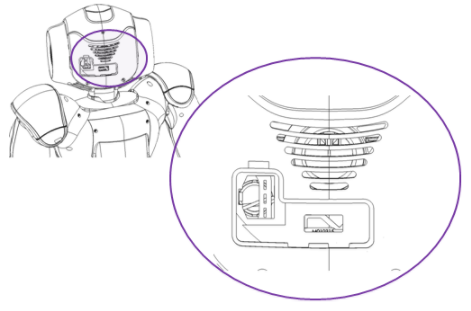
\includegraphics[width=110mm]{Bilder/Mert/Klappe.png}
				\caption{Die zu entfernende Klappe hinter dem Kopf des Roboters}
				\label{Klappe hinter dem Kopf des Roboters}
				\end{figure}						
			
			
	\subsection{Interaktion}
	\subsection{Sensoren}
		\subsubsection{FSRs}
			FSR steht für Force Sensitive Resistors. Sozusagen Kraftempfindliche 
			Widerstände. Diese wiederstände messen den Widerstandsunterschied entsprechend 
			dem angewandten Druck. Diese FSR sind auf den Füßen des Roboters positioniert 
			und arbeiten in einem Bereich von 0 N bis 25 N.
			\begin{figure}[h]
			\centering
			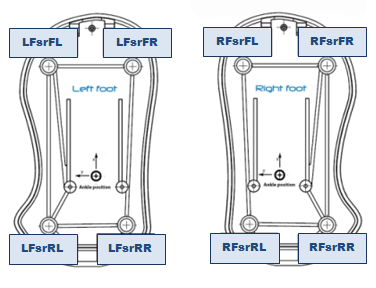
\includegraphics[width=110mm]{Bilder/Mert/FSR.jpg}
			\caption{FSR-Positionen im Knöchelrahmen}
			\label{FSR-Positionen}
			\end{figure}			
		\subsubsection{Trägheitseinheit}
		\subsubsection{Ultraschallsensoren}
		\subsubsection{Gelenkpositionssensoren}
		\subsubsection{Kontakt- und Tastsensoren}
	\subsection{Kinematikdaten}
		\subsubsection{Verbindungen}
		\subsubsection{Gelenke}
		\subsubsection{Massen}
		\subsubsection{Motoren}
			
	



\newpage
\null\vfill
\begin{center}
 \part[Praktischer Teil]{\centering Praktischer Teil} 
\end{center}
\vfill
\newpage

\section{Erste Einstellungen des Roboters}
	\subsection{Das erste Einschalten}
	






\newpage
\listoffigures
\end{document}
